%%%%%%%%%%%%%%%%%%%%%%%%%%%%%%%%%%%%%%%%%%%%%%%%%%%%%%%%%%%%%%%%%%%%%%%%%%%%%%%%
% This covers the problem analysis portion of the thesis
%
%%%%%%%%%%%%%%%%%%%%%%%%%%%%%%%%%%%%%%%%%%%%%%%%%%%%%%%%%%%%%%%%%%%%%%%%%%%%%%%%

\chapter{Problem Analysis}
A purely abstract visualization may not be the best data representation if
the underlying data has inherently physical/spatial dimensions. In this chapter, we discuss why
this is the case. Here, we also present our use case dataset of vehicle complaint
documents, which we will use through out the remainder of this thesis.
 

%This chapter proposes our alternative approach for navigating a large body of
%text. In particular, we introduce our dataset and problem domain: exploring 
%vehicle complaint reports for reliability and safety analysis. We introduce our
%goals and our requirement gathering process. Lastly we take a closer look at
%our dataset records and specify the dimensions we want to visualize to support
%our goals.

    % ===== Figure =====
	\begin{figure}
       \begin{center} 
       \begin{tabular}{c}
       \framebox[1\width ]{
       \begin{tabular}{l}
       The car is wandering sideways and you have to really control and \\
       focus on keeping the wheel straight to stay on lane. The best way \\
       to describe it is like you are always driving on windy weather \\
       with severe wind gusts. This happens on highway, with a speed of 60 \\
       MPH or higher. The assistant service manager said it could be the \\
       wheel alignment but after they aligned it and checked it, the problem \\
       remains. I live in an area where we get significant amount of snow \\
       during winter and I am afraid of my safety because of this problem. \\
       \end{tabular}
       } \\
       \end{tabular}
       \end{center}	
 	   \caption{An example of a complaint summary text.}
	   \label{figure:complaint}
	\end{figure}
	% ==================

%   % ===== Figure =====
% 	\begin{figure}
% 	   \centering  
% 	   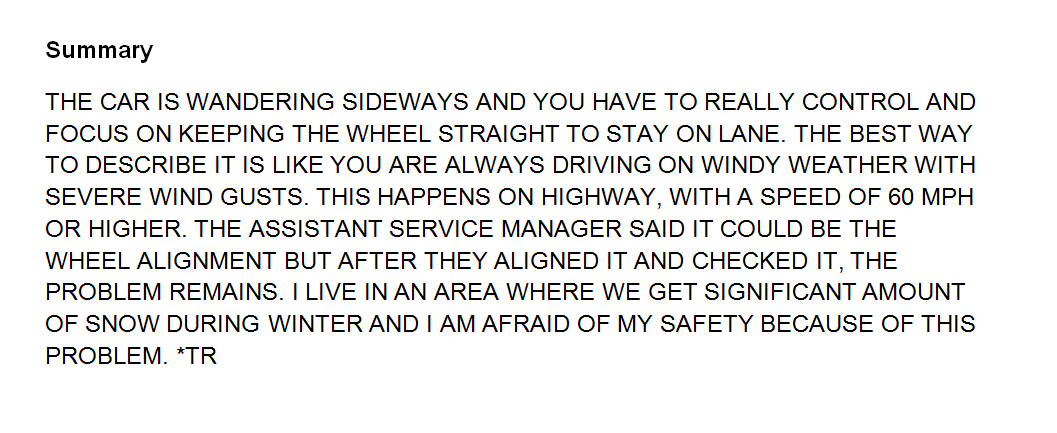
\includegraphics[width=\columnwidth]{complaint_text.png}
% 	   \caption{An example of a complaint summary}
% 	   \label{figure:complaint}
% 	\end{figure}
% 	% ==================


\section{Problem}
When it comes down to navigating, exploring and querying large bodies of text,
traditional visualization techniques often approach the problem from an abstract
perspective. These techniques explore the context of words in the sentence of
the documents. For example Word Tree~\cite{Wattenberg2008} allows people to
explore the most frequently occurring sentence structures within a document.
Other types of visualization look at summarizing the underlying text: popular 
visualizations on the web today such as tag-clouds and word-cloud emphasize
the most frequently occurring words or phrases, thus revealing possible themes in
the text. Still, other techniques look at the language semantics, for example 
DocuBurst spatially organizes words based on the ``IS-A''
relationship~\cite{COL2009a}.

Looking at the underlying semantics helps us understand the content and 
themes in the text documents. However, there is another type of word context 
that is not fully explored in the visualization community. Within any text 
document which describes physical objects, each word that describes a 
tangible object has relation to its physical, real-world counterpart. The 
entities also have relation to each other in terms of their respective 
spatial positions. For example, the sentence ``Automatic door locks when 
used, will not release from any of the four doors when engine is turned off.'' 
contains not only a co-occurrence relationship among the entities ``door'' and 
``engine,'' but also relates to where the doors and engine are located on a 
real-world automobile.

% Revealing these spatial relations of common words in text may enable new types of 
% insights and exploration techniques. By mapping physical entities onto virtual
% \threed representations it is possible to create a visualization environment
% that resembles the real world, the environment can then be explored and queried with relative ease
% due to existing familiarity of how these objects operates in real life. There are 
% many types of text that carries these sort of physically mappable vocabulary: 
% product reviews, technical manuals, maintenance logs, and our dataset: vehicle 
% defect reports.

Revealing the spatial dimensions has several potential benefits. Foremost, the
familiarity of the form makes the subject matter immediately recognizable
to experts and novices alike. Exploration of data can leverage previous 
experiences with the subject matter, using visual examination of graphics 
rather than reading textual data. Second, it is possible to conduct a different
type of data exploration: the spatial dimension allows us to explore
proximal relations and filter by spatial volumes, possibly allowing
new insights to be formed.

So far, we are not aware of any exploratory visualization which approaches text
analytics by visualizing the real-world spatial context of the words in
text. Thus, our work looks at revealing these real-world relations in a manner
that is useful for conducting text-analytic activities. By preserving the physical
attributes in the text documents, and combining them with NPR illustration style 
rendering, we argue that this approach creates a rich and engaging experience.

Consider product quality reports for a musical instrument such as the trumpet.
Visualizing these reports could allow one to see the exact location of the problems on the
\threed model, such as which valves are failing. Seeing the instrument
in physical form may promote conjectures that are less apparent
with text or abstract visualization, for example, perhaps the valves
failed because they are encased in a faulty housing. There are many
applicable datasets which carry this sort of physically mappable vocabulary:
consumer product reviews, technical manuals, and technical
support logs are examples.
 


\section{Use Case: Vehicle Complaint Reports}
We choose to demonstrate our approach on a dataset of vehicle complaint
reports. Each year thousands of reports are submitted to the
NHTSA database, consisting of consumer complaints, defect reports
and manufacturer recalls. Each report has fixed fields describing the
details of the incident (date, make, model, etc.), and a free-form text
field, typically containing several sentences which describe the incident
in detail, including what physical parts were damaged or broken. A sample of the
text description, which we use to drive our visualization, can be seen in Figure
\ref{figure:complaint}.  Collectively, the metadata and free
text offer a wealth of information on safety and reliability issues of
vehicles. Consumers can access this data online to support car-buying
decisions. The current interface (see Figure \ref{figure:nhtsa}) uses a
conventional search form, returning long lists of textual results; there are no mechanisms to support
concise overviews or dynamic details-on-demand. 

    % ===== Figure =====
	\begin{figure}
	   \centering  
	   \includegraphics[width=\columnwidth]{nhtsa_website.png}
	   \caption[NHTSA Complaint search interface]{NHTSA Complaint search
	   interface~\cite{nhtsa}.}
	   \label{figure:nhtsa}
	\end{figure}
	% ==================



\subsection{Requirements and Tasks}
% We start our initial requirement gathering by looking what people say, and
% how they use vehicle safety related information. Our sources includes websites 
% dedicated to vehicle owners and potential car buyers, expert columns, 
% question and answer forums, car-buying tips and product rating websites such 
% as Consumer Reports\footnote{http://www.consumerreports.org/} and
% Edmunds\footnote{http://www.Edmunds.com}. 

We start our initial requirement gathering by looking at what people say, and
how they use vehicle safety related information. Our sources include websites 
dedicated to vehicle owners and potential car buyers, expert columns, 
question and answer forums, car-buying tips and product rating websites such 
as Consumer Reports~\cite{consumerReports} and Edmunds~\cite{edmunds}. Data
collection was done manually by browsing forum posts and annotating the types of
questions being asked; for the product rating sites we noted what type of things
they gave a grade to and how they were rated.


Our findings revealed that safety and reliability is a big concern, next to
vehicles prices. In general, people want to know which brand/make 
they can trust. Forum posts referred to vehicle issues, with existing owners 
asking whether the problems are isolated events or if the issues are widely
spread, this indicates a need and willingness for detailed exploration. Finally, car buying 
guides often advocate conducting thorough research on the vehicle and brand history, 
as well as leverage the experience of other owners. 
 
Based on these findings, we propose the following four design requirements for
our visualization prototype:
\begin{itemize}[noitemsep]
  \item R1: Provide an intuitive representation and make important items clearly
  visible;
  \item R2: Facilitate finding of trends, interesting facts and causal relations
  in the reports;
  \item R3: Allow multiple types of comparisons across different data
  dimensions; and
  \item R4: Provide for reading of original complaint report text in the context
  of the visualization.
\end{itemize}

% The types of tasks that we want to support are based on Rohrdanz \etal's seven
% important analytical tasks for dealing with streaming data~\cite{ROH2011a}. 
% Though the vehicle complaint dataset is not real-time it is temporal in nature
% and shares many of the same concerns as real-time applications. Some sample 
% tasks are:


The types of tasks we want to support are based on the seven analytical tasks for streaming 
data from Rohrdanz \etal.~\cite{ROH2011a}. Though the vehicle complaint dataset is not real-time it is temporal in nature
and shares many of the same concerns as real-time applications. Some sample 
tasks are:

\begin{itemize}[noitemsep]
   \item Decision Making: Which vehicle should I buy? Are there enough
   reports and evidences to warrant a full scale investigation or a recall?
   \item Historical Retrieval: Are there any major concerns with vehicle X over the last five years?
   \item Exploration: How does vehicle X compare to other vehicles in the same category?
   \item Monitoring: Are there any new complaints relating to vehicles of make Y?
   \item Change and Trend Detection: For this type of vehicle, are the rate of complaints per month increasing or decreasing?
\end{itemize}


%\section{Summary}
%There are many text collections that deal with physical data, 